%%%%%%%%%%%%%%%%%%%%%%%%%%%%%%%%%%%%%%%%%%%%%%%%%%%%%%%%%%%%%%%%%%%%%%%%%%%%%%%%
%2345678901234567890123456789012345678901234567890123456789012345678901234567890
%        1         2         3         4         5         6         7         8

\documentclass[letterpaper, 10 pt, conference]{ieeeconf}  % Comment this line out if you need a4paper
\usepackage[T1]{fontenc}
\usepackage{booktabs}
\usepackage{cite}

%\documentclass[a4paper, 10pt, conference]{ieeeconf}      % Use this line for a4 paper

\IEEEoverridecommandlockouts                              % This command is only needed if 
                                                          % you want to use the \thanks command

\overrideIEEEmargins                                      % Needed to meet printer requirements.

%In case you encounter the following error:
%Error 1010 The PDF file may be corrupt (unable to open PDF file) OR
%Error 1000 An error occurred while parsing a contents stream. Unable to analyze the PDF file.
%This is a known problem with pdfLaTeX conversion filter. The file cannot be opened with acrobat reader
%Please use one of the alternatives below to circumvent this error by uncommenting one or the other
%\pdfobjcompresslevel=0
%\pdfminorversion=4

% See the \addtolength command later in the file to balance the column lengths
% on the last page of the document

% The following packages can be found on http:\\www.ctan.org
%\usepackage{graphics} % for pdf, bitmapped graphics files
%\usepackage{epsfig} % for postscript graphics files
%\usepackage{mathptmx} % assumes new font selection scheme installed
%\usepackage{times} % assumes new font selection scheme installed
\usepackage{amsmath} % assumes amsmath package installed
%\usepackage{amssymb}  % assumes amsmath package installed
\usepackage[dvipsnames]{xcolor}
\usepackage{bbding}
\usepackage{pifont}
\usepackage{wasysym}
\usepackage{amssymb}
\usepackage[pdftex]{graphicx}
\usepackage{multicol}
\usepackage{colortbl}
\usepackage{hyperref}
\usepackage{url}
\usepackage{multirow}
\usepackage{tabularx}
\usepackage{mathtools}
\usepackage{xcolor}
\usepackage[nolist]{acronym}
\usepackage{amssymb}% http://ctan.org/pkg/amssymb
\usepackage{pifont}% http://ctan.org/pkg/pifont
\newcommand{\cmark}{\ding{51}}%
\newcommand{\xmark}{\ding{55}}%
%\newcommand{\HIU}[1]{\textcolor{cyan}{HIU: #1}}
%\newcommand{\HAK}[1]{\textcolor{orange}{ HAK: #1}}
%\newcommand{\OLA}[1]{\textcolor{blue}{OLA: #1}}
%\newcommand{\JON}[1]{\textcolor{green}{JON: #1}}




%% ORCID
\RequirePackage{tikz} % For \foreach used for Orcid icon
% Make Orcid icon
\newcommand{\orcidicon}{\includegraphics[width=0.32cm]{figures/logo-orcid.eps}}

% Define link and button for each author
\foreach \x in {A, ..., Z}{%
\expandafter\xdef\csname orcid\x\endcsname{\noexpand\href{https://orcid.org/\csname orcidauthor\x\endcsname}{\noexpand\orcidicon}}
}

\definecolor{Bookcolor}{HTML}{00F9DE}
\definecolor{darkgreen}{rgb}{0.0, 0.5, 0.0}

\newcommand{\orcidauthorA}{0000-0001-5387-7613} % Add \orcidA{} behind the author's Hakim
\newcommand{\orcidauthorB}{0000-0003-3581-9481} % Add \orcidB{} behind the author's Olaya
\newcommand{\orcidauthorC}{0000-0002-1609-5783} % Add \orcidC{} behind the author's name  Halil
\newcommand{\orcidauthorD}{0000-0002-7742-6996} % Add \orcidD{} behind the author's name  Jonas
\newcommand{\orcidauthorE}{0009-0002-0445-8126} % Add \orcidE{} behind the author's name  Yury
\newcommand{\orcidauthorF}{0000-0002-7143-8777} % Add \orcidF{} behind the author's name  Erdal


\DeclareMathOperator*{\minimize}{{min}}
\DeclareMathOperator*{\maximize}{{max}}



%acronyms
\begin{acronym}
    \acro{ROV}{remotely operated vehicle}
    \acro{AUV}{autonomous underwater vehicle}
    \acro{UWRS}{underwater robotics simulator}
    \acro{NMPC}{nonlinear model predictive control}
    \acro{MPC}{model predictive control}
    \acro{SLAM}{simultaneous localisation and mapping}
    \acro{vSLAM}{visual SLAM}
    \acro{RL}{reinforcement learning}
    \acro{DRL}{deep reinforcement learning}
    \acro{UE}{unreal engine}
    \acro{NED}{North-East-Down}
    \acro{UE5}{unreal engine 5}
    \acro{UE4}{unreal engine 4}
    \acro{ROS}{robot operating system}
    \acro{AI}{artificial intelligence}
    \acro{APE}{absolute positioning error}
    \acro{RPE}{relative positioning error}
    \acro{PWM}{pulse width modulation}
    \acro{DFKI}{Deutsches Forschungszentrum für Künstliche Intelligenz}
\end{acronym}





\title{\LARGE \bf
UNav-Sim: A Visually Realistic Underwater Robotics Simulator and Synthetic Data-generation Framework
}


\author{ 
Abdelhakim Amer\orcidA{}, Olaya Álvarez-Tuñón\orcidB{}, Halil \.{I}brahim U\u{g}urlu\orcidC{}, Jonas le Fevre Sejersen\orcidD{}, \\ Yury Brodskiy\orcidE{} and
Erdal Kayacan\orcidF{}% <-this % stops a space
% <-this % stops a space
\thanks{A. Amer, O. Tunon, H. U\u{g}urlu, J. Sejersen  are with the Department of Electrical Engineering and Computer Engineering, Aarhus University, 8200 Aarhus, Denmark {\tt\small \{abdelhakim, olaya, halil, jonas\} at ece.au.dk}.
Y. Brodskiy is with EIVA a/s, 8660 Skanderborg, Denmark. {\tt\small \{ybr\} at eiva.com}.
E. Kayacan is with the Automatic Control Group, Department of Electrical Engineering and Information Technology, Paderborn University, Paderborn, Germany. {\tt\small \{erdal.kayacan\} at uni-paderborn.de}}
}
\begin{document}



\maketitle
\thispagestyle{empty}
\pagestyle{empty}


%%%%%%%%%%%%%%%%%%%%%%%%%%%%%%%%%%%%%%%%%%%%%%%%%%%%%%%%%%%%%%%%%%%%%%%%%%%%%%%%
\begin{abstract}
%Underwater robotics tests are expensive due to the complex working environment and requirement for various sensor modalities in the underwater domain. Even though underwater simulators are a must, the rendering quality of many existing simulators is inadequate, limiting their ability to transfer algorithms from simulation to real-world applications. We introduce UNav-Sim, to overcome this limitation. To the best of our knowledge, UNav-Sim is the first simulator to incorporate the efficient, high-detail rendering of unreal engine 5 (UE5). It is open-source\footnote{\url{https://github.com/Zartris/ColosseumUnderWater}} and includes an autonomous control and vision-based navigation framework. Furthermore, Hydr-Sim makes use of AirSim's advanced features, such as its efficient physics solver and diverse sensor models, including GPS, IMU, cameras, and sonar. To enable communication between the autonomy framework and the physics simulator, an API can be utilized in either C++ or Python to transfer essential sensor data and issue control commands. Additionally, the C++ client library can be interfaced with a ROS wrapper, enabling researchers to efficiently develop and test their algorithms underwater and transfer them to real-world systems. 

%, it suppor enabling researchers to efficiently develop and test their algorithms underwater and transfer them to real-world systems. 

%Marine robotics simulators are essential for advancing robotics research as they enable rapid algorithm testing without the cost and complexity of real-time experiments. In addition, they can provide accurate positioning data, which is often unavailable in the real world. However, the rendering quality of many existing simulators is inadequate, limiting their ability to transfer algorithms from simulation to real-world applications. To overcome this limitation, we introduce \ac{UWRS}, a new simulator for autonomous underwater robotics research that extends the popular drone simulator AirSim. \ac{UWRS} is the first simulator of its kind to incorporate the efficient, high-detail rendering of \ac{UE5}. It is open-source and includes an autonomous control and vision-based navigation framework, enabling researchers to efficiently develop and test their algorithms and transfer them to real-world systems.

i just checked hallowen is only this week%Underwater robotics surveys can be expensive due to the complex working environment and the need for various sensor modalities. Although underwater simulators are essential, many existing simulators have inadequate rendering quality, which limits their ability to transfer algorithms from simulation to real-world applications. 

Underwater robotic surveys can be costly due to the complex working environment and the need for various sensor modalities. While underwater simulators are essential, many existing simulators lack sufficient rendering quality, restricting their ability to transfer algorithms from simulation to real-world applications. To address this limitation, we introduce UNav-Sim, which, to the best of our knowledge, is the first simulator to incorporate the efficient, high-detail rendering of Unreal Engine 5 (UE5). UNav-Sim is open-source\footnote{\url{https://github.com/open-airlab/UNav-Sim}} and includes an autonomous vision-based navigation stack. By supporting standard robotics tools like ROS, UNav-Sim enables researchers to develop and test algorithms for underwater environments efficiently.% It also facilitates the easy transfer of these algorithms from simulation to real-world systems.
\end{abstract}


%%%%%%%%%%%%%%%%%%%%%%%%%%%%%%%%%%%%%%%%%%%%%%%%%%%%%%%%%%%%%%%%%%%%%%%%%%%%%%%%
\section{Introduction}
\label{sec:introduction}

% % Underwater Robot Applications:
%
In many applications, \Acfp{ROV} play a pivotal role, including surveying, inspection, and search-and-rescue operations, by improving efficiency and ensuring safety \cite{amer2023unav, amergp}.
%
% Why We Need Tether:
%
Most \acp{ROV} are tethered to ensure a continuous power supply during long-duration missions and to maintain reliable communication.
%
% Introducing Problem Definition:
%
However, the presence of a tether introduces complexities in path planning and control, as it poses a risk of entanglement with underwater objects such as flora, fauna, or structures being inspected.

This challenge restricts the applicability of many path planning algorithms originally designed for untethered drones and surface vehicles. For instance, numerous \ac{CPP} algorithms exist to compute distance-optimal paths for covering 3D structures \cite{bircher2015structural,feng2024fc, amer2023visual}. Additionally, exploration path planners are employed to determine the next viewpoints for mapping and exploring unknown terrains \cite{dang2020graph}. However, these methods do not account for entanglement with the surroundings and thus cannot be directly applied to tethered underwater robots.
%
% Entanglement Problem and Definition:
%
Entanglement occurs when the movement of the underwater vehicle is restricted due to physical interactions between the tether and objects in the environment. Tether can bend or loop around obstacles, limiting vehicle mobility. This work bridges a critical gap in automatic asset inspection with \ac{ROV} by proposing \ac{REACT}.

The contributions of this work can be summarized as follows:
\begin{itemize}
\item A fast online tether model that computes the tether configuration in real time using \ac{SDF} data of arbitrary underwater structures.
\item An efficient online replanning method that prevents entanglement by incorporating a maximum tether length constraint.
\item Integration of the proposed method into a coverage path planning framework with \ac{MPC} to enable optimal inspection of underwater structures while avoiding entanglement.

\item Demonstration of the complete framework in simulation, showcasing its ability to ensure safe and efficient underwater structure inspection.
\end{itemize}





%
\begin{figure}[t!]
	\centering	\includegraphics[width=0.7\linewidth]{figures/react_abstract.pdf}
	  \caption{\textcolor{black}{Overview of the \ac{REACT} inspection framework. In the offline phase, a \ac{SDF} map is generated from a point cloud, and the FC-Planner \cite{feng2024fc} computes an optimal waypoint sequence. In the online phase, a tether model $\mathbf{P}^{tether}(t)$ ensures the maximum tether length is maintained, while an \ac{MPC} controller applies the optimal wrench $\mathbf{u}(t)$ to the \ac{ROV}}.}
    \label{fig:abstract}
\end{figure}
%


The remainder of this paper is organized as follows: Section \ref{sec:related_work} reviews the state of the art. Section \ref{sec:framework} presents the path planning framework for underwater structure inspection with tether constraints. Section \ref{sec:tether_model} introduces the taut-tether model, and Section \ref{sec:planner} details the online entanglement-aware path planner. Experimental results are shown in Section \ref{sec:experiments}, followed by conclusions and future work in Section \ref{sec:conclusion}.






\input{sections/2-state_of_the_art.tex}
\input{sections/3-simulator_description.tex}
\input{sections/4-robotics_stack.tex}
\section{Example use-cases}\label{sec:tests}
As a case study for UNav-Sim, we present an autonomous pipe inspection scenario. 
%We have used pre-existing assets from the unreal engine marketplace to construct the simulation environment. This modular approach represents a straightforward and adaptable method for simulation environment construction.
Pipe inspection, being the most common use case for \ac{ROV}s, presents a relevant and challenging use case, where vision-based navigation is essential to achieve the required task. Furthermore, we assess the efficacy of our underwater autonomy stack and report its performance in executing the designated autonomous pipe inspection task. A video showing the pipe inspection demonstration can be found here\footnote{\url{https://youtu.be/unZS33lCqpU}}.



\subsection{Vision-based pipe following with DRL}\label{sec:example:planning}

In this experiment, the performance of UNav-Sim is evaluated in a pipe-following task. An agent utilizing \ac{DRL} is trained with the gym interface provided by the simulator to generate position commands based on RGB image observations. An \ac{MPC} controller subsequently executes the position commands. The convolutional neural network policy inputs $180\times320$ pixel RGB image observation, $o_t$, from a downward-looking camera on \ac{ROV} and outputs an action, $a_t$, describing one meter away waypoint consisting of two values, $a_1, a_2 \in [-1, 1]$. The actions represent the direction of the position step and turn in the heading angle, respectively, similar to our previous work \cite{halil}. The reward is defined with respect to vertical divergence from the pipe unless the termination of episodes; $r_t = 10 - 2e_p^2 - 2e_\psi$ where $e_p$ is the closest distance to the pipe in the horizontal plane and $e_\psi$ is the error in heading with respect to pipe direction. An episode is terminated where the pipes are not in the camera's field of view, which is $e_p > 2.5 m$. The \ac{DRL} agent is trained with proximal policy optimization~\cite{schulman2017proximal} algorithm using \texttt{stable-baselines3}~\cite{stable-baselines3} package.

The trained policy is deployed on a pipe $\sim20$ meters long with right and left turns. The trajectory of the agent along with the pipes is visualized in Fig. \ref{fig:trajectory_drl}.
While the agent is not accurately tracking the pipes due to the exploratory behavior of the \ac{DRL} policy, it learns to make reasoning from image observations and successfully follows the pipe.
This experiment demonstrates the utilization of high-fidelity image observations and accurate dynamics provided by UNav-Sim in a particular application.

\begin{figure}[t]
    \centering
    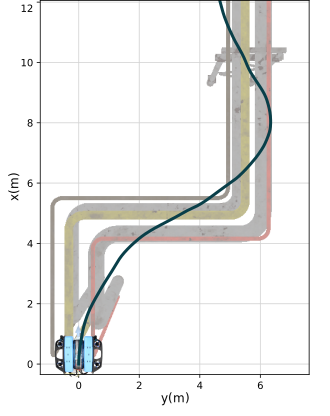
\includegraphics[width=8.4cm]{figs/paper5-unavsim/trajectory2.pdf}
    \caption[Trajectory drawn by the ROV in the DRL experiments]{Trajectory followed by the \ac{DRL} agent (dark blue) along with the pipes from the top view. The starting point is the origin of the coordinate frame and is indicated with the \ac{ROV}.
    %The  experimental results show that training the ego agent (\ac{ROV}) in a photo-realistic underwater environment can effectively enable it to be deployed in an underwater pipe inspection scenario.
    }
    \label{fig:trajectory_drl}
\end{figure}



\subsection{Visual localization benchmarking}
The vision-based trajectory generated in Section \ref{sec:example:planning}, being carried out by the robot with the controller showcased in Section \ref{sec:stack:control}, has served as a test setup for the visual localization experiment.
Two trajectories are carried out: a linear trajectory where no area in the map is revisited (see Fig. \ref{fig:trajectory_drl}), and a trajectory with a loop, where the robot navigates back to the starting point.
The benchmarking is automatically performed by the \texttt{robot\_visual\_localization} metapackage using \cite{grupp2017evo}. 

During runtime, the estimated trajectory $P_i$ and the ground truth trajectory $Q_i$ are recorded into separate files composing a sequence of time-synchronized spatial poses. The pose format is the one proposed in \cite{sturm2012tumrgbd}, composed of the three spatial coordinates with the orientation in quaternions.
The metrics implemented are the \ac{APE} and the \ac{RPE}, which are automatically deployed over the recorded trajectories before shutdown. TartanVO presents a monocular visual odometry algorithm. Therefore, for a fair comparison, the ORB-SLAM3 experiment is executed under a monocular setup. 
The deployment of monocular algorithms implies that the orientation of the algorithm's world frame and the trajectory's scale is arbitrary. Therefore, the estimated trajectories are aligned with the ground truth by obtaining the transform $S \in Sim_3$ that best aligns $P_i$ with $Q_i$.

With the deployment of the automatic stack for visual inspection proposed by UNav-Sim, benchmarking of visual localization algorithms becomes a straightforward task: the robot follows the pipeline autonomously under the planned trajectory, with the visual localization algorithms being automatically executed by the \texttt{robot\_visual\_localization} package, which on shutdown generates the results as depicted in Table \ref{unavsim:table:comparisonSLAM}. It can be seen from the generated results that the two proposed algorithms depict a similar performance in the linear trajectory, but ORB-SLAM outperforms TartanVO under the presence of a closed loop.
Despite ORB-SLAM's high efficiency in state-of-the-art datasets, the realistic underwater conditions confront one of the main challenges for feature-based approaches: the lack of texture. Moreover, the pipes are the main source of features, which avoids their uniform distribution across the image. Without enough evenly-distributed features, the ORB-SLAM's front end drifts. Nevertheless, the closed trajectory shows the convenience of the back-end's loop closure algorithm: the absolute errors are significantly reduced for translation and rotation.
On the other hand, TartanVO presents a drift similar to ORB-SLAM's in the translations, but slightly higher for rotations. These results show the great potential of learning-based algorithms under imaging conditions that challenge geometry-based methods. Although the lack of generalization ability is the main source of drift in this case, TartanVO has been trained with high amounts of diversified data that explain its good performance in the proposed setup.

In conclusion, the framework proposed in UNav-Sim has enabled the automatic benchmarking of state-of-the-art visual localisation algorithms in a realistic underwater scenario. This has allowed the challenges and opportunities of these algorithms to be easily demonstrated in a geometry-based and learning-based manner.

\begin{table}[ht!]
\centering
\footnotesize
\caption[Visual localization results in the pipeline tracking scenario]{Visual localization results in the pipeline tracking scenario.}
\label{unavsim:table:comparisonSLAM}
\begin{tabular}{cc c c c c  }
\toprule

Trajectory                   & Algorithm  & APE[m]         & RPE[m]         & APE[rad]       & RPE[rad] \\
\midrule
\multirow{2}{*}[0em]{Linear} & ORB-SLAM3  & 1.75          & \textbf{0.412} & \textbf{1.53} & \textbf{0.036} \\
                             & TartanVO   & \textbf{1.67} & 0.489          & 1.95          & 0.108 \\
\midrule
\multirow{2}{*}[0em]{With loop}   & ORB-SLAM3  & \textbf{0.078}          & 0.372 & \textbf{1.62} & \textbf{0.006} \\
                             & TartanVO   & 0.961 & \textbf{0.322}         & 2.10          & 0.068 \\
\bottomrule
\end{tabular}
\end{table}

% \begin{table}[ht!]
% \centering
% \scriptsize
% \caption{visual localization results in the pipeline tracking scenario.
% }
% \label{unavsim:table:comparisonSLAM}
% \begin{tabular}{|c| c c c c | }
% \hline

% Algorithm  & APE[m]         & RPE[m]         & APE[rad]       & RPE[rad] \\
% \hline
% ORB-SLAM3  & 1.754          & \textbf{0.412} & \textbf{1.525} & \textbf{0.036} \\
% TartanVO   & \textbf{1.667} & 0.489          & 1.952          & 0.108 \\
% \hline
% \end{tabular}
% \end{table}




\section{Conclusion \& future work} \label{sec:unavsim:conclusion}
We have developed UNav-Sim, a novel open-source underwater simulator, which builds upon AirSim and \ac{UE5} and incorporates state-of-the-art robotics algorithms. UNav-Sim also supports \ac{ROS} and multiple operating systems, facilitating a streamlined and efficient development process for robotics applications. Future work will include the incorporation of additional underwater sensors, vehicle models, and more custom environments. 





% \addtolength{\textheight}{-12cm}   % This command serves to balance the column lengths
                                  % on the last page of the document manually. It shortens
                                  % the textheight of the last page by a suitable amount.
                                  % This command does not take effect until the next page
                                  % so it should come on the page before the last. Make
                                  % sure that you do not shorten the textheight too much.

%%%%%%%%%%%%%%%%%%%%%%%%%%%%%%%%%%%%%%%%%%%%%%%%%%%%%%%%%%%%%%%%%%%%%%%%%%%%%%%%



%%%%%%%%%%%%%%%%%%%%%%%%%%%%%%%%%%%%%%%%%%%%%%%%%%%%%%%%%%%%%%%%%%%%%%%%%%%%%%%%



%%%%%%%%%%%%%%%%%%%%%%%%%%%%%%%%%%%%%%%%%%%%%%%%%%%%%%%%%%%%%%%%%%%%%%%%%%%%%%%%
%\section*{APPENDIX}


\section*{Acknowledgement}
This work is supported by EIVA a/s and Innovation Fund Denmark under grants 2040-00032B and 1044-00007B, the European Union’s Horizon 2020 Research and Innovation Program (OpenDR) under Grant 871449 and the Marie Skłodowska-Curie (REMARO) under Grant 956200. This publication reflects the authors’ views only. The European Commission is not responsible for any use that may be made of the information it contains.

%%%%%%%%%%%%%%%%%%%%%%%%%%%%%%%%%%%%%%%%%%%%%%%%%%%%%%%%%%%%%%%%%%%%%%%%%%%%%%%%


%. 1044-00007B



\bibliographystyle{unsrt}
\bibliography{refs}
\end{document}
